\chapter{Introduction}

Until the release of Dungeon Keeper\footnote{Bullfrog Productions, 1997} most well known fantasy 
video games have allowed the player to play as various heroic characters, raiding dungeons filled
with evil forces in order to aquire treasures and fame.
In Dungeon Keeper, however, we join the opposite faction and try to defend our own dungeon
(along with all the treasures hidden in it) from endless hordes of heroes trying to pillage our domain.
Although we can still play the original Dungeon Keeper today, we cannot change its data or game mechanics
in any easy way so this thesis aims to recreate and modify the original game and extend it to have an easy to 
use programming interface that will allow such modifications.

\section{Dungeon Managment Genre}

Dungeon Keeper was the first game released in the dungeon management~(DM) genre and since our game is going to be based on
Dungeon Keeper, we should design it with the elements of its genre in mind. Since the definition of this genre has to our
knowledge never been formally documented by the creators of Dungeon Keeper, we are going to create a list of basic elements
of the genre based on the gameplay of the original game.

In Dungeon Keeper, the player's main goal is to build and protect his own base, called the dungeon. They do so by commanding
their underlings (often called minions), whom they can command to mine gold, which is a resource they use in order to build new rooms
and cast spells (in the game's sequel\footnote{Dungeon Keeper 2, Bullfrog Productions, 1999}, mana was added into the game
as a secondary resource used for spell casting), which could be researched as the game progressed. They would then use creatures
spawned in their buildings as well as their own magic powers to fight intruders in order to protect their dungeon. 
From this brief gameplay summary, we can create list of the most basic design elements, which can be found in dungeon management games:

\begin{enumerate}[label=\textbf{(E\arabic*)}]
    \item Resource management
    \item Dungeon building
    \item Minion commanding
    \item Combat
    \item Player participation in combat
    \item Research
\end{enumerate}

Now that we have created a list of the genre's basic design elements, let us have a look at how they were implemented in games from the
Dungeon Keeper series.

\subsubsection{Resource management}

In the original Dungeon Keeper, the player used gold as their primary resource. They would have it mined by their minions and use
it to build new rooms and cast spells. While having a single resource for everything may bring simplicity to the game, it also means
that once the player runs out of gold, they wont be able to directly participate in combat due to their inability to cast spells.
It is for this reason that we are going to use the resource model of Dungeon Keeper 2 and have a separate resource -- mana -- that
will be used to cast spells.

\bigskip
Ask PJ: Should the word mana be itallic in the same way mods and modding tools are? This is its second appearance in the text, but the
first one wasn't "definitioney" and a general player should know the concept.

\subsubsection{Dungeon building}

The term dungeon building in Dungeon Keeper refers to tearing down walls in order to create new rooms which the player's minions 
then claim and the player can place new buildings in. These buildings can then act as gold storage, spawn new creatures or be used
as traps that negatively affect attacking enemies. Since this is a central theme in Dungeon Keeper (and dungeon management games
in general), we should try to implement our building model to resemble this.

\subsubsection{Minion commanding}

The term minion commanding stands for giving your minion tasks such as to move somewhere, attack an enemy or tear down a wall. In
Dungeon Keeper, most of these commands were implemented as spells -- although mining was done by simply selecting blocks, which
could unfortunately cause minions to destroy walls the player accidentally selected. To providea unified interface to minion tasks
and to avoid the accidental block destruction, all commands the player can give will be in our game implemented as spells.


\subsubsection{Combat}

In Dungeon Keeper, the player's dungeon is under frequent attacks by enemy heroes. These enemies attack the dungeon 
in groups with a delay between each two attacks, in a similar way to tower defense games (e.g. Orcs must die!~\cite{OMD} 
and Dungeon Defenders~\cite{DungeonDefenders}), where theay are often referred to as \emph{waves}. Each wave of enemies
can consist of different types of heroes and the delay between ways can differ, too. Since the players of the original
Dungeon Keeper are alredy familiar with this wave system and it also caters to players of tower defense games, we will be
implementing it in our game.

\subsubsection{Player participation in combat}

During the fights with enemy heroes, the player in Dungeon Keeper can cast various spells to affect the outcome of the battle.
These spells can have various forms from spawning creatures, damaging enemies and healing minions to destroying walls and throwing
meteors. If we want to create a similar spell system, we need to support these different types of spells, e.g. targeted spells that
affect a single entity, positional spells that can summon a creature or global spells, that simply have an effect on the game once
they are cast.

\subsubsection{Research}

In the original Dungeon Keeper, researching new spells and buildings was done through a special type of room, called the library,
which can be seen in Figure~\ref{dk-lib}. There,
various minions could study and achieve new advancements for the player after a certain amount of research points -- which was different
for different spells and buildings -- was gathered. But this design decision brought a negative element into the game, because once the
library was destroyed by the heroes, the player was unavailable to perform additional research and could even use the ability to cast
some spells. This is why we are going to use a different approach, called the research tree (or sometimes technology tree), first used
in the real-time stragety game called Sid Meyer's Civilization\footnote{Developed by MPS Labs, 1991}~\cite{ResearchTrees}. This approach 
separates the research from the events happening in the game and allows the player to research new advancements for a resource (e.g. gold),
with each new technology, building, creature or spell being able to have prerequisites.

\begin{figure}[h]
    \centering
    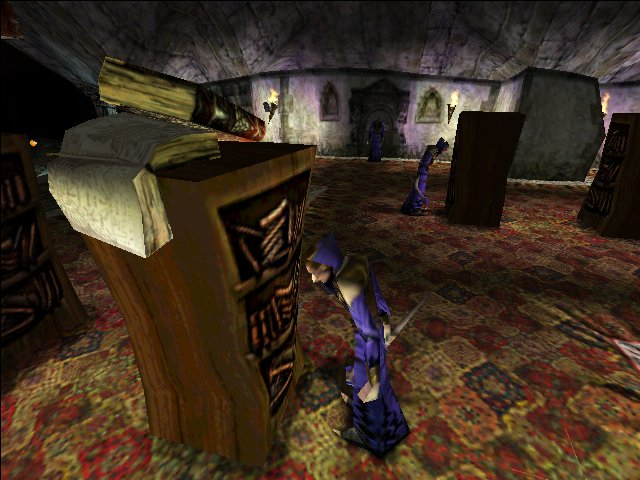
\includegraphics[width=10cm]{../img/library.jpg}
    \caption{Warlocks researching in the library.
             \\Source: \href{http://vignette2.wikia.nocookie.net/dungeonkeeper/images/9/98/Library.jpg/revision/latest?cb=20120808211437}{http://dungeonkeeper.wikia.com}}
    \label{dk-lib}
\end{figure}

\subsubsection{Conclusion}

We have now investigated the main design elements of Dungeon Keeper (and dungeon management games in general) and how we are going 
to implement them in our game. The last thing we have to realise is that since we are trying to cater to the players of the original
game, the resulting product of our work should be a full game and not just a prototype. This means that the game should offer full 
singleplayer experience, with relatively intelligent enemies and the ability to not only win the game, but to also lose. It also means
that the game has to be performant, achieving atleast the minimum acceptable framerate, defined as 25-30 frames per second by 
Shiratuddin, Kitchens and Fletcher~\cite{AcceptableFPS}, on both new and older hardware.

\section{Modifiability in Games}

One of our basic goals is for our game to be modifiable, which means to provide tools -- often called \emph{modding tools} -- to our players
that will allow them to create modifications -- often called \emph{mods} -- that other players can install and which can change or
add elements to the game.

This can increase the replay value of the game as after finishing it, more missions, characters, game mechanics, abilities, items
or even game modes can be easily downloaded and installed from internet. Since we want our game to be modifiable, we should allow our players
to change most (if not all) of the game's data, artificial intelligence and abilities of all minions, creatures and enemies and also give
them the ability to edit levels the game, which would allow them to create new maps.

An important topic we need to decide on is which parts of the game we will allow the players to modify. 
An example of an easily modifiable game is Minecraft~\cite{Minecraft}, a 3D sandbox game 
in which the player has to survive in a procedurally generated world, which can be seen in Figure~\ref{minecraft}. 
The player builds a house, crafts tools, mines for materials and
fights off enemies during the night. These elements of the game provide a wide array of things that mods can change. For example to smelt
ores into ingots, the player can use a furnace powered by coal, but a mod called Industrial Craft~2~\cite{IndustrialCraft} added machines
into the game that, among other uses, could smelt ingots using electricity, another concept introduced by the mod. The player can then
create power plants of different types -- ranging from solar to nuclear -- to produce electricity that they can then use to power their
machines. With this mod, the player can create setups that allow him to automate tasks such as smelting, cooking or mining. An example of
such setup can be seen in Figure~\ref{ic-solar}.

\begin{figure}[h]
    \centering
    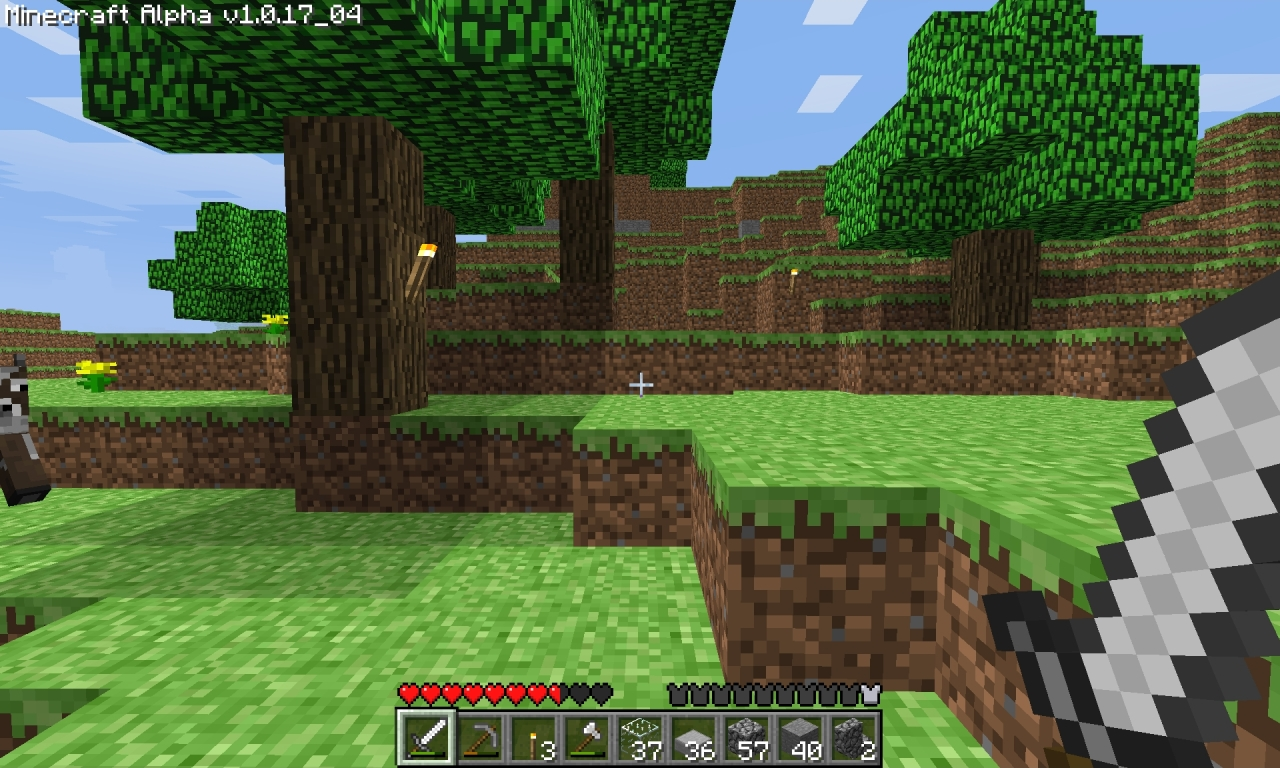
\includegraphics[width=10cm]{../img/minecraft.jpg}
    \caption{A procedurally generated world in Minecraft.
             \\Source: \href{http://i.neoseeker.com/p/Games/PC/Simulation/City/minecraft\_image\_zx2AU2n6bZho0lz.jpg}{http://www.neoseeker.com}}
    \label{minecraft}
\end{figure}

\begin{figure}[h]
    \centering
    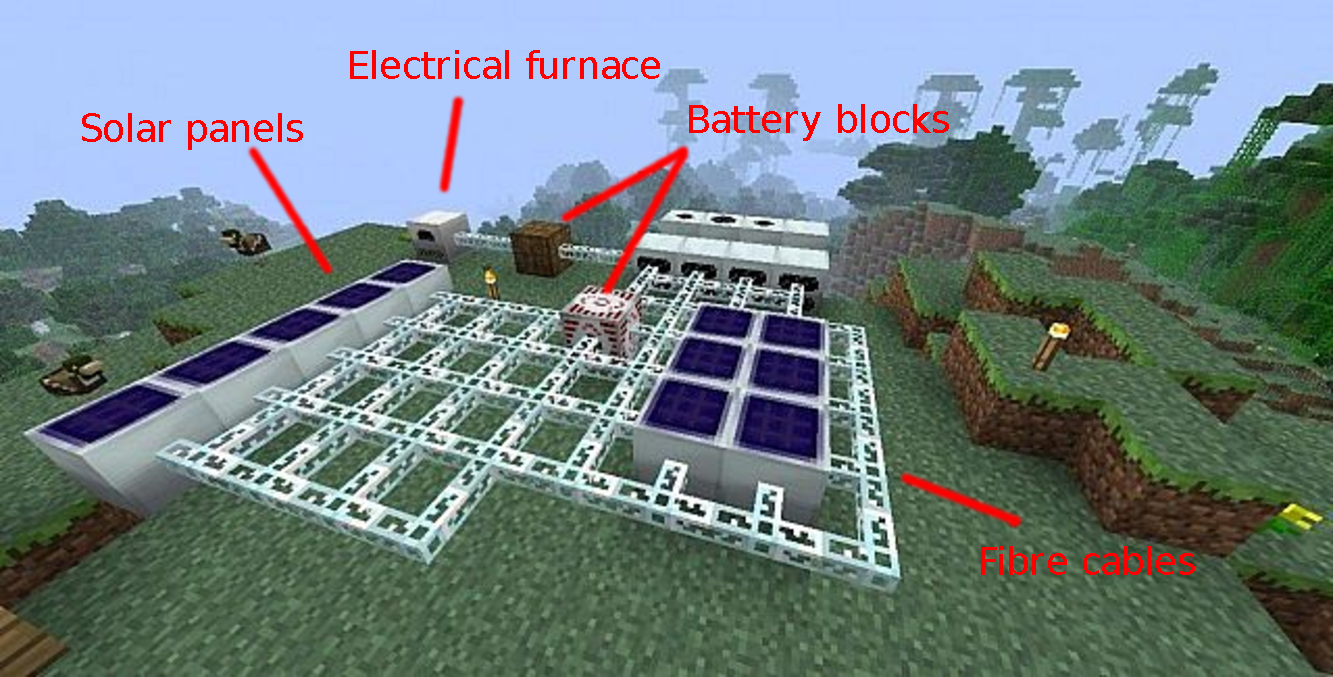
\includegraphics[width=10cm]{../img/ic-solar.pdf}
    \caption{A simple setup powering multiple machines including an electrical furnace using solar panels.
             \\Source: \href{http://static.planetminecraft.com/files/resource\_media/screenshot/1246/javaw-2012-11-12-20-51-09-46\_4122139.jpg}{http://www.planetminecraft.com}}
    \label{ic-solar}
\end{figure}

Another mod, called ComputerCraft~\cite{ComputerCraft}, added fully functional computers into the game. 
These computers can be used to create password protected
doors, write programs and games in Lua or even connect to internet services such as IRC\footnote{Internet Relay Chat, an open communication 
protocol.}. An example of such computer in minecraft can be seen in Figure~\ref{computer-craft}. This mod also added robots into the game, 
that could be programmed using Lua scripts to automate tasks such as mining, fighting or woodcutting.

\begin{figure}[h]
    \centering
    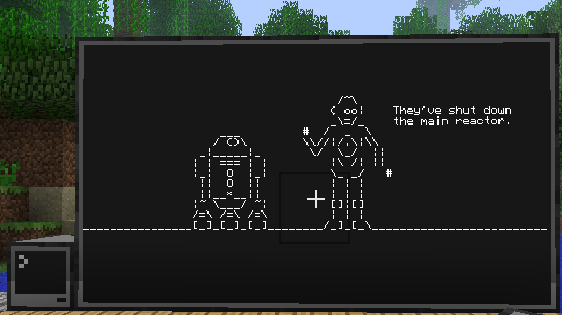
\includegraphics[width=10cm]{../img/ComputerCraft2.png}
    \caption{A computer in Minecraft playing the ASCII version of the movie Star Wars: A New Hope.
             \\Source: \href{http://minecraft-modding.de/wp-content/uploads/2015/06/ComputerCraft2.png}{http://www.minecraft-modding.de}}
    \label{computer-craft}
\end{figure}

In Minecraft, the player has access to simple tools, e.g. a pickaxe or a sword, but with mods, the game can be ehnanced with advanced 
technologies or even magic (e.g. Thaumcraft or MineMagicka). This can create new ways the game is played and possibly extend its
replayability.

Aside from adding items and creatures, entire new games can be created within a modifiable game. For example Minecraft's command block,
which can execute commands in the game's developer console -- e.g. teleport the player to a certain position or give him items --
when interacted with, was used by a player of the game to create~\cite{FutureOfMinecraft} a custom map that copied the game 
Team Fortress~2~\cite{TF2}. Team Fortress~2 is a 3D first person shooter, in which two player teams fight against each other in various
game modes, e.g. capture the flag, deathmatch or point control. Each player could choose from a wide selection of character classes, 
each with its
own attributes and weapons. The command block was used for example to equip players based on the character class they choose -- 
which can be done by choosing between different command blocks each being assigned to a single class and a console command that 
adds an item to a player -- or controlling a point, for which a command block can check if a player stands on a point long enough
to capture it.

\bigskip
Ask PJ: Should I explain the terms CTF, DM and point controol? Most players should already know them :/
\\Also, when I mentioned Thaumcraft and MineMagicka, the only official resources are their forum posts which have long urls
and can change them over time (updating patch version in the post title alters the url -.-), should I refer to them anyway?
\bigskip

To allow the creation of custom maps in our game, we should store our levels
in a format that will allow later modifications, including actual changes to the game's elements.

In conclusion, we can see that the ability to modify a game can help said game to grow even when its development has stopped
or is focused in different areas (e.g. security, stability). Since we want to give this ability to the players of
our game, our modding tools should allow them to change most of its data, including but not limited to:

\begin{itemize}
    \item Minions and enemies -- e.g. changing attributes such as health and damage, displayed models, behavior and spells they
        cast.
    \item Buildings -- e.g. changing their size, models, types of creatures that they spawn and, in the case of traps, their interaction with
        enemies.
    \item Spells -- fully changing the effect of a spell, e.g. from simple damage dealing to spawning a meteor shower.
    \item Goals of the game -- changing requirements for winning the game or the reasons for a loss.
\end{itemize}

Besides changing data of entities -- e.g. creatures, buildings or spells -- the players should also be able to create new types of these
entities.

The game on its own should also be fully featured, offering enough of these entities
on its own so the players do not need mods to actually play the game. Additionally, since our game, like Dungeon Keeper,
will have scripted waves of enemies attacking the player's dungeon, the also should allow our players to alter the wave 
composition -- that is, which types of enemies compose the different groups attacking the player's dungeon --  and delays between
the waves. Last, but not least, we must not forget that players do not necessarily have to be (and often are not)
programmers, so our game should provide an easy way to install these modifications.

\section{Thesis Goals}

The main goal of this thesis is to design and implement a modifiable 3D dungeon management game using the design elements \textbf{(E1)}~--~\textbf{(E6)}.

In addition to the main goal, the game should complete the following list of goals:

\begin{enumerate}[label=\textbf{(G\arabic*)}]
    \item The game has to be a full competetive product, not a prototype.
        \begin{enumerate}[label=\textbf{(G1.\arabic*)}]
            \item It has to be performant, achieving high framerate even on low end computers.
            \item It has to offer full single player experience, with scripted enemies and a chance to both win and lose.
            \item It has to contain a variety of entities, spells and buildings even without mods.
        \end{enumerate}
    \item The game has to be highly modifiable, providing an easy to use modding interface for players.
        \begin{enumerate}[label=\textbf{(G2.\arabic*)}]
            \item The mod creators must be able to create new entities, spells and buildings and to change most of the game's data.
            \item They must also be able to alter the game progression by defining enemies that spawn and delays between them.
            \item The game should also support the creation of custom levels.
        \end{enumerate}
    \item The mods for the game have to be easily installable even by players without any programming knowledge. 
\end{enumerate}
